\begin{multicols}{2}
\byline{Ученическият съвет}{Калина 10В}

Учениците в ГПНЕ ”Гьоте” са много активни в различни области. Като възпитаници на Немската гимназия, те поддържат и утвърждават авторитета и. За да се насърчава развитието на учениците в гимназията са им предоставени множество извънкласни дейности.

Като израз на демократичния дух на управление и възпитание на учениците преди 15 години е създаден ученическият съвет като форма на демократична изява на мнението на учениците.

След основаването си от Вида Ангелова той не е спирал да функционира. Негова основна цел е да сформира ядро от будни и иновативни ученици, които да дават предложения и да изразяват мнение,  да помага на учителския колектив и ръководството, да организира тържества и най-важото - да продължава традициите на гимназията. Организиране на тържества и базари, провеждане на „Мис и Мистър Подготве” и Fashing и посещения на Защитено жилище „Акациите” и Социален център град Бургас са част от ежегодните събития.

И нека не забравяме, че зад  развитието и успехите на ученическия съвет стои ръководството и директорите на гимназията.
\end{multicols}

\begin{center}
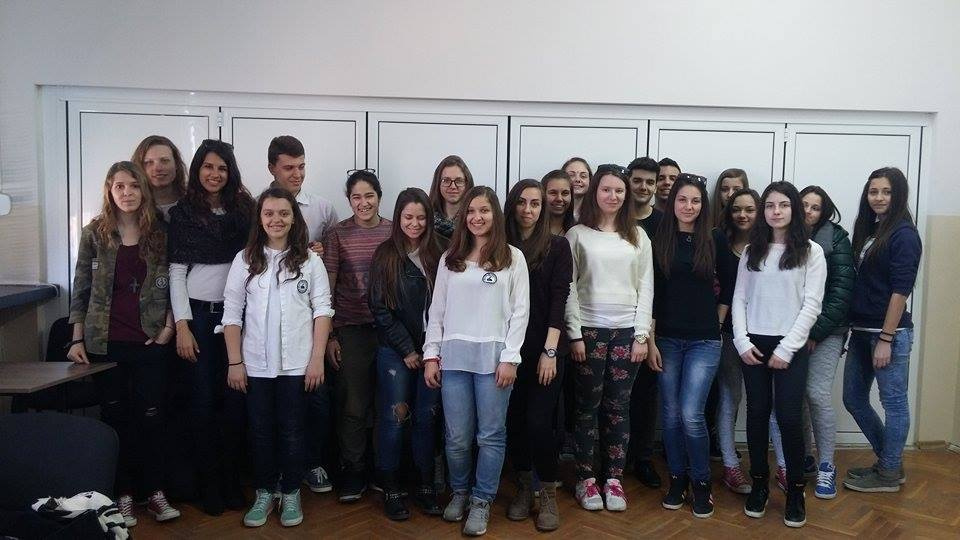
\includegraphics[width=6.0in]{./US/US.jpg}\\
\end{center}
\closearticle
